\begin{frame}
  \frametitle{关键字}
  \begin{itemize}
    \item 定义:事先定义的,有特别意义的单词,被Java语言保留下来有着特殊含义和用途,所以有时又叫保留字
    \item 所由的Java关键字都是小写
    \item \texttt{goto}和\texttt{const}虽目前未被Java使用,但是依旧是保留关键字
    \item 一般情况下,IDE编辑器会将关键字以特殊高亮的形式展现
  \end{itemize}
  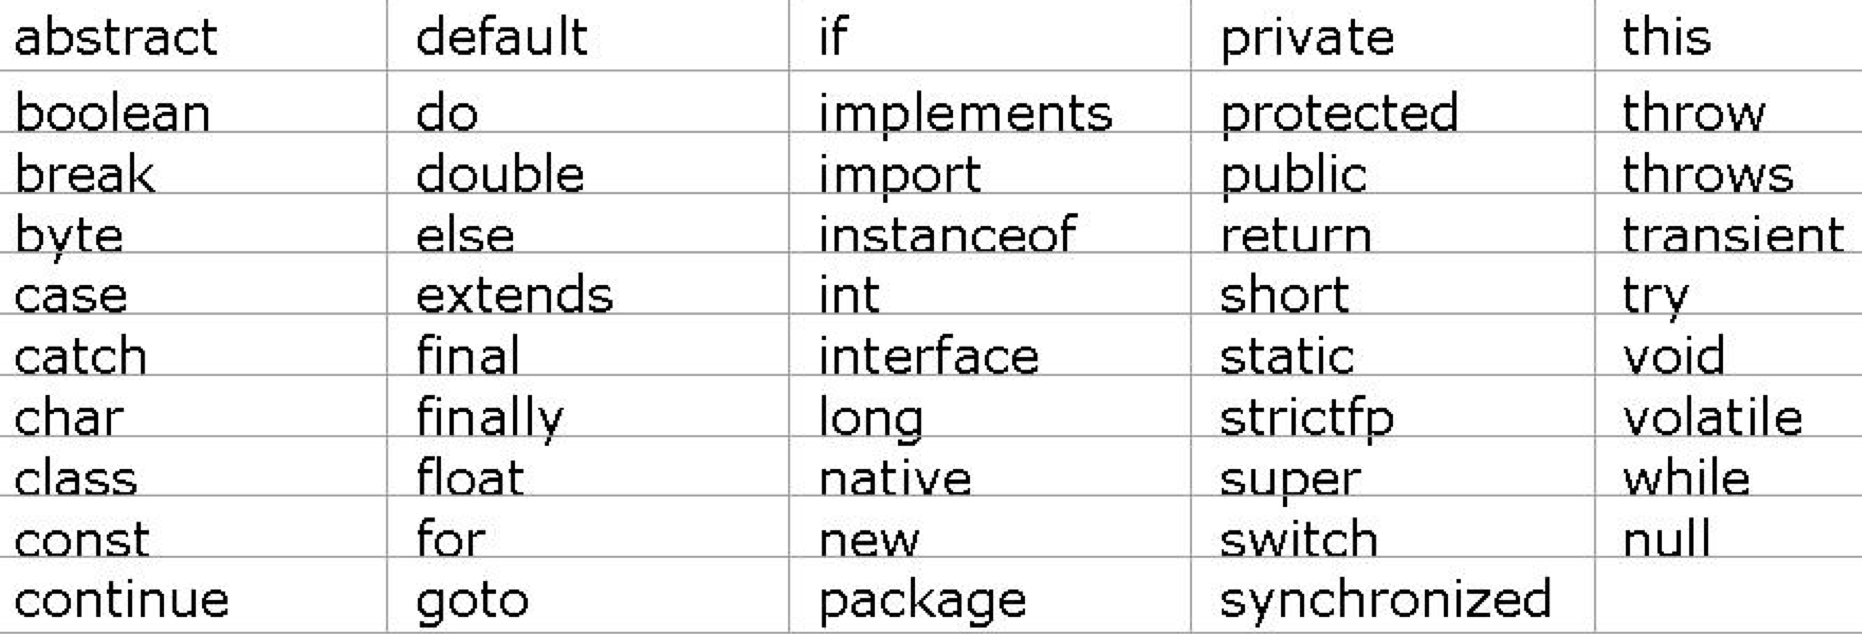
\includegraphics[width=\textwidth]{figures/keywords}
\end{frame}

\begin{frame}
  \frametitle{标识符}
  \begin{itemize}
    \item 定义:用于给Java程序中变量、类、方法等要素命名的字符串序列
    \item Java标识符规则:
      \begin{itemize}
        \item 只能由字母、数字、下划线“\_”、美元符"\$"号组成
        \item 不能以数字开头,只能以字符、下划线、美元符号开头
        \item 不能是Java中的关键字
        \item 大小写敏感
      \end{itemize}
    \item 通俗地说,凡是可以自己起名字的地方,都要遵守标识符规则
    \item 标志符中的字母指Unicode中的字母,不光包括英文26个字母,甚至包括中文的汉字、希腊字母、日文片假名等
    \item 合法标志符举例:\texttt{myName,My\_name,Points,\$points,\_sys\_ta,OK,\_23b,\_3\_}
    \item 非法标志符举例:\texttt{\#name,25name,class,\&time,if}
  \end{itemize}
\end{frame}

\begin{frame}[fragile]
  \frametitle{变量}
  \begin{itemize}
    \item 变量是Java中最基本的数据存储单元,其要素包括:变量名、变量的数据类型和作用域
    \item 变量必须先声明,后使用,声明格式为:\java|type varName [= valValue]|
    \begin{javacode}
      String a; //声明了一个变量,但未赋值,相当于C中的空指针
      int i = 100; //声明了一个变量,并为其赋值
      double a, b, c = 1.1; //一次赋值三个变量
    \end{javacode}
    \item 本质上讲,Java中的变量其实就是内存中的一小块区域,这块区域可以使用变量名来访问
  \end{itemize}
\end{frame}

\begin{frame}
  \frametitle{Java中的数据类型}
  \begin{itemize}
    \item Java中共两大类数据类型:基本数据类型和引用数据类型
    \item 引用数据类型实际就是C语言中的指针引用!Java中除了基本数据类型,其它本质上都是指针!
    \item Java函数的参数如果是基本数据类型,那么传值调用;如果是引用类型,则本质上是传址调用!
  \end{itemize}
  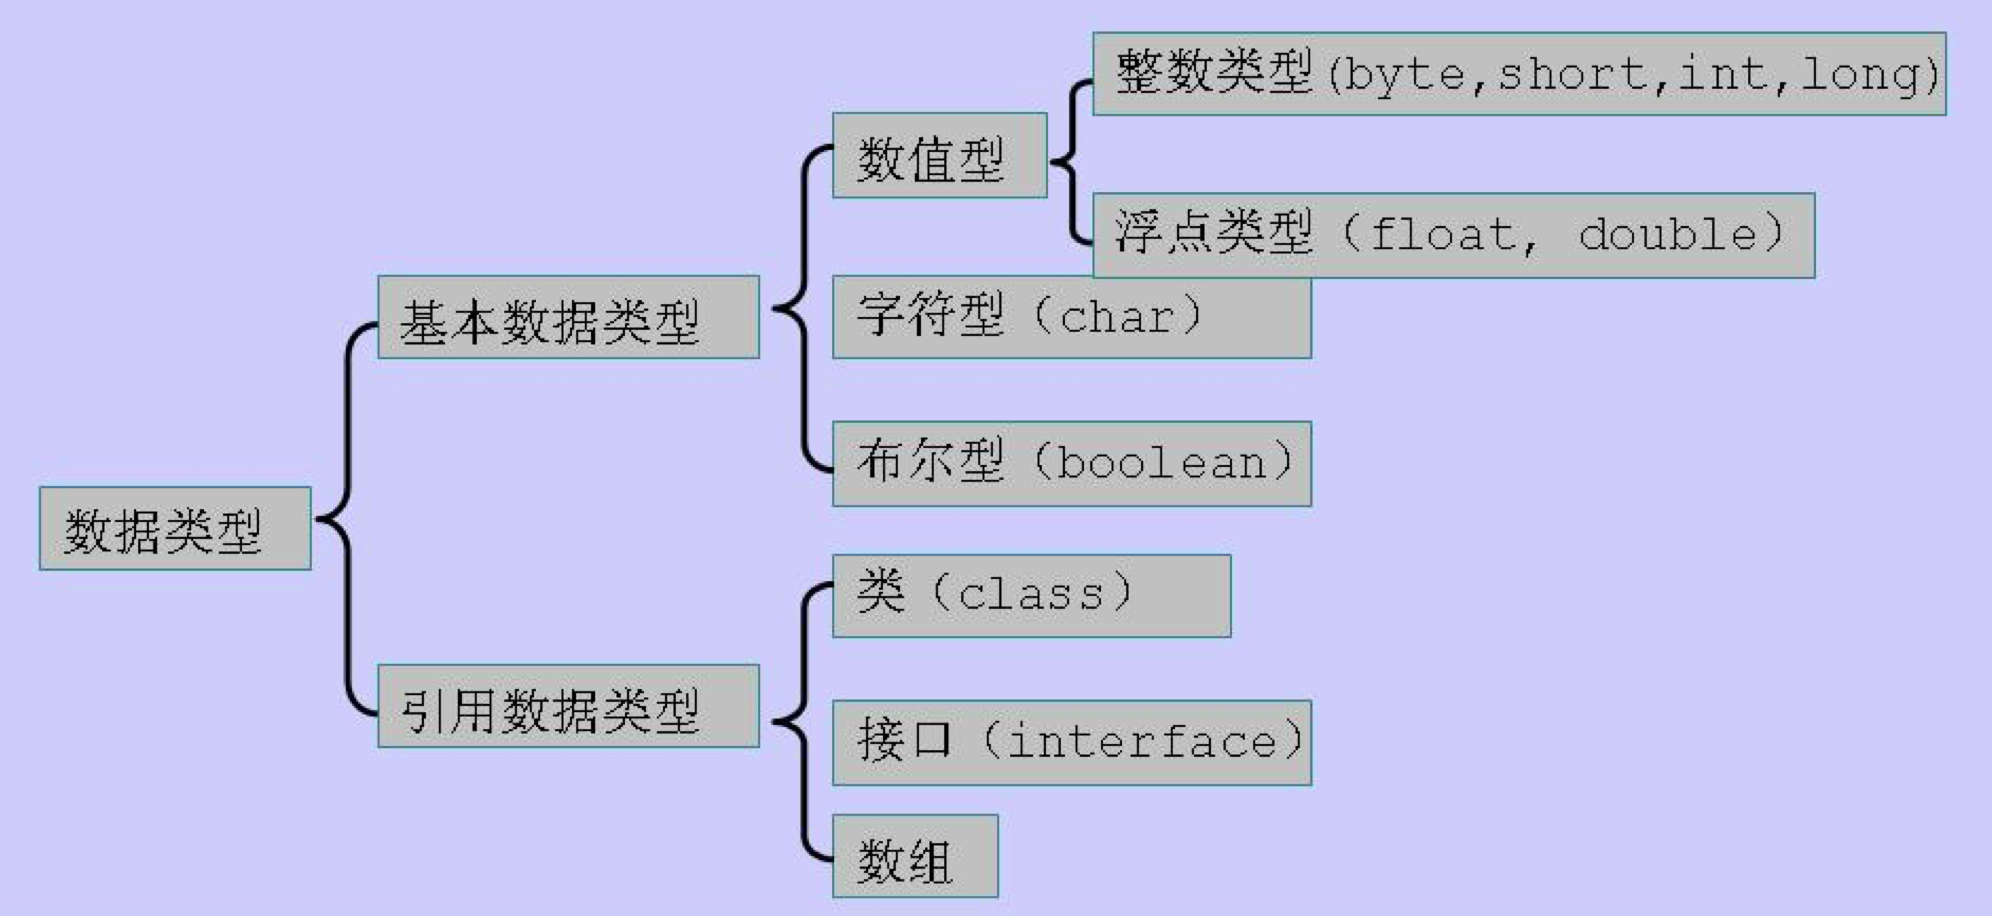
\includegraphics[width=\textwidth]{figures/data_types}
\end{frame}


\begin{frame}[fragile]
  \frametitle{布尔型}
  \begin{itemize}
    \item 布尔型数据用于逻辑运算,一般用于程序流程控制,使用\texttt{boolean}声明一个布尔型变量
    \item Java中的布尔型数据只能取两个值\texttt{true}和\texttt{false},不能使用0或者null来表示(注意此处和和C语言不同)
  \end{itemize}
  \begin{javacode}
    boolean a = true;
    boolean b = false;
    
    if (a) { //使用布尔型数据用于流程控制
    }
    
    boolean c = 0; //错误,Java中布尔型只能取true或者false
    
    int d = -1;
    if (d) { //错误,Java中只能使用布尔型做为程序流程控制
    }
  \end{javacode}
\end{frame}

\begin{frame}[fragile]
  \frametitle{字符型}
  \begin{itemize}
    \item 字符型数据表示一个字符,用单引号\texttt{'}包围(注意不能用双引号,双引号包围的是字符串!)
    \item Java字符采用Unicode编码,每个字符占用两个字节,所以字符类型数据可以转换为整数型数据
    \item Unicode编码的字符不光包含了Asic字符,还包含了很多外语的字母,如汉字等
    \item 允许使用反斜杠来表示具有特殊意义的字符
  \end{itemize}
  \begin{javacode}
    char a = 'x';
    char b = "x"; //错误,双引号括起来的表示字符串
    char c = 'abc'; // 错误,字符型数据只能是1个字符
    char d = '\n'; //表示一个换行符
    char e = '1';// e是一个字符型数据,不是一个整数!
    char f = '中'; //Java中的字是Unicode编码的字符,包括中文
    char f = '\u0061'; // 采用Unicode的形式给字符赋值
  \end{javacode}
\end{frame}

\begin{frame}
  \frametitle{数组}
  \begin{itemize}
    \item 数组是多个\textbf{相同}类型数据的集合
    \item 和C语言中的数组类似,Java中的数组本质上也是一个指针,属于Java的引用类型,做为函数参数是进行传址调用
    \item 声明方式:\java|type valName[]|
  \end{itemize}
\end{frame}